\documentclass[12pt, titlepage]{article}

\usepackage{fullpage}
\usepackage[round]{natbib}
\usepackage{multirow}
\usepackage{booktabs}
\usepackage{tabularx}
\usepackage{graphicx}
\usepackage{float}
\usepackage{longtable}
\usepackage[flushleft]{threeparttable}
\usepackage{hyperref}
\usepackage{placeins}
\graphicspath{ {./} }
\hypersetup{
    colorlinks,
    citecolor=black,
    filecolor=black,
    linkcolor=red,
    urlcolor=blue
}
\usepackage[round]{natbib}

\newcounter{acnum}
\newcommand{\actheacnum}{AC\theacnum}
\newcommand{\acref}[1]{AC\ref{#1}}

\newcounter{ucnum}
\newcommand{\uctheucnum}{UC\theucnum}
\newcommand{\uref}[1]{UC\ref{#1}}

\newcounter{mnum}
\newcommand{\mthemnum}{M\themnum}
\newcommand{\mref}[1]{M\ref{#1}}
\begin{document}


\title{\textbf{SE 3XA3: \\Module Guide\\CraftMaster}}

\author{\textbf{Group Number: }307\\
		\textbf{Group Name: }3 Craftsmen \\
		\textbf{Members: }\\
		Hongqing Cao 400053625\\
		Sida Wang	 400072157\\
		Weidong Yang 400065354}

\date{}

\maketitle
\newpage

\pagenumbering{roman}
\tableofcontents
\listoftables
\listoffigures
\newpage

\begin{table}[!htbp]
\begin{tabularx}{\textwidth}{llX}
\toprule
\textbf{Date} & \textbf{Editor(s)} & \textbf{Change}\\
\midrule
Mar 9 & Sida & General Content added\\
Mar 13 & Weidong & Edited for Rev0 submission\\
Mar 13 & Sida & Minor Modification\\
Apr 6 & Sida & Completed for Rev1\\
Apr 6 & Hongqing & Final Check\\
\bottomrule
\end{tabularx}
\caption{\textbf{Revision History}} \label{TblRevisionHistory}
\end{table}


\newpage

\pagenumbering{arabic}

\section{Introduction}
The format of this document follows the template provided by Dr.Bokhari and Thien Trandinh.
\subsection{Project Overview}
CraftMaster is a re-implementation of \href{https://github.com/fogleman/Minecraft}{\textbf{Michael Fogleman's Simple Minecraft-inspired Demo}} (referred to as \textbf{original project} in the following content), which is developed in Python and Pyglet. The CraftMaster design team has initiated and completed multiple requirements(specified in the \href{https://gitlab.cas.mcmaster.ca/wangs132/minecraft/-/blob/master/Doc/SRS/SRS.pdf}{\textbf{Software Requirement Specifications(SRS)}}) to add new features, including new block types, day and night mode shift, game saving, and game menu frames, to the original project. During the software design process, the team has also applied software architecture design patterns and software design principles to increase the quality of the software design. The specification of those design methodologies will be described in this document.\\\\
In terms of the software product characteristics, CraftMaster is a 3D Sandbox Game that allows players to control the character and build the game world based on their imagination. We believe that CraftMaster will be beneficial to teenagers and children in the way that it inspires them to unleash their creativity. 

\subsection{Context of Module Guide}
The \href{https://gitlab.cas.mcmaster.ca/wangs132/minecraft/-/blob/master/Doc/SRS/SRS.pdf}{\textbf{SRS}} document shows the features, functionalities and desired properties that the system should have.
The \textbf{Module Guide(MG)} is generated based on the \href{https://gitlab.cas.mcmaster.ca/wangs132/minecraft/-/blob/master/Doc/SRS/SRS.pdf}{\textbf{SRS}}, which further evaluates how requirements are achieved and also specifies the modular structure decomposition of the software system. It will be distributed to help potential readers easily identify the decomposed parts of the software. The potential readers are as follows:
\begin{itemize}

    \item \textbf{New Project Members:} The \textbf{MG} acts as a guideline for the new project members to easily and quickly understand the modular structure of the system and its decomposition specifications. With this document, those new members can search for relevant modules more efficiently.
    \item \textbf{Designers:} The \textbf{MG} is used to help software system designers check for the consistency among modules, the flexibility of the design, and the feasibility of the modular decomposition.
    \item \textbf{Developers:} The hierarchical structure specified in the \textbf{MG} will give the developers a better understanding of the system decomposition and use relationships between different modules.
    \item \textbf{Maintainers:} The hierarchical structure of the system improves the maintainers' understanding of either the system as a whole or individual modular parts when they need to make changes to the system and the documents.
\end{itemize}
The \href{https://gitlab.cas.mcmaster.ca/wangs132/minecraft/-/blob/master/Doc/Design/MIS/MIS.pdf}{\textbf{Module Interface Specifications(MIS)}} is another section of the Design Specifications Documents other than the \textbf{MG}. The \href{https://gitlab.cas.mcmaster.ca/wangs132/minecraft/-/blob/master/Doc/Design/MIS/MIS.pdf}{\textbf{MIS}} shows the semantics and syntax of exported functions for each module in details. The \textbf{MG} should be an entry document for the design specifications and the readers should read the \textbf{MG} first to get an overview of the system, then browse the \href{https://gitlab.cas.mcmaster.ca/wangs132/minecraft/-/blob/master/Doc/Design/MIS/MIS.pdf}{\textbf{MIS}} for further references once they identify which module(s) they are searching for.

\subsection{Design Principles}
\begin{itemize}
    \item \textbf{High Cohesion and Low Coupling}: This principle has been applied to the project in the way that the modules are designed to be strongly related and the dependency has been minimized.
    \item \textbf{Open-Closed Principle}: The modules are designed to be closed to modification and the system is designed to easily extended. For instance, the \href{https://gitlab.cas.mcmaster.ca/wangs132/minecraft/-/blob/master/src/screen.py}{\bf screen} module is implemented as a template and all other scenes(such as \href{https://gitlab.cas.mcmaster.ca/wangs132/minecraft/-/blob/master/src/gameScene.py}{\bf gameScene}, \href{https://gitlab.cas.mcmaster.ca/wangs132/minecraft/-/blob/master/src/mainScene.py}{\bf mainScene} and \href{https://gitlab.cas.mcmaster.ca/wangs132/minecraft/-/blob/master/src/settingScene.py}{\bf settingScene}) inherit it. There might be new scenes to be implemented in the future to easily extend the system.
    \item \textbf{Liskov Substitution Principle}: The inheritance relationships among modules follows the Liskov Substitution Principle.
    \item \textbf{Dependency Inversion Principle}: The inheritance design pattern is used to support the abstraction of the system. With the abstraction, the dependency inversion principle can be followed.
    \item \textbf{Interface Segregation Principle}: The inheritance design pattern minimizes the interfaces of subclass modules, which follows the Interface Segregation Principle.
    \item \textbf{Law of Demeter}: The abstraction of the system supports the principle of the Law of Demeter. The communications only depend on the interfaces as limited knowledge.
    \item \textbf{Information Hiding}: The information hiding principle is supported by abstraction and private methods.
\end{itemize}

\subsection{Content Structure}

The rest of the document is organized as follows:
\begin{itemize}

\item Section \ref{SecChange} lists the anticipated and unlikely changes of the software
requirements. 
\item Section \ref{SecMH} summarizes the module decomposition that
was constructed according to the likely changes. 
\item Section \ref{SecConnection}
specifies the connections between the software requirements and the
modules. 
\item Section \ref{SecMD} gives a detailed description of the
modules. 
\item Section \ref{SecTM} includes two traceability matrices. One checks
the completeness of the design against the requirements provided in the SRS. The
other shows the relation between anticipated changes and the modules. 
\item Section
\ref{SecUse} describes the use relation between modules.
\end{itemize}


\subsection{Naming Conventions and Terminology}
The naming conventions and terminology section will aid readers from different backgrounds to clearly understand the content of this document. The naming conventions and terminologies used in this document are listed below:
\begin{itemize}
        \item \textbf{OS:} Operating System.
        \item \textbf{GUI:} Graphical User Interface, which allows the user to interact and visualize the program by graphics instead of text.
        \item \textbf{Sandbox Game:} A type of game that allows player to create, modify, and destroy the environment.
        \item \textbf{Pyglet:} The Python library for the design of graphical user interface and multi-media.
        \item \textbf{Player/Gamer:} The person who controls the PC to play the game.
        \item \textbf{Character:} The fictional character who is controllable by the player/gamer(not visible to the player).
        \item \textbf{3D Game:} A game in three dimensions.
\end{itemize}

\section{Anticipated and Unlikely Changes} \label{SecChange}

This section lists possible changes to the system. According to the likeliness
of the change, the possible changes are classified into two
categories. Anticipated changes are listed in Section \ref{SecAchange}, and
unlikely changes are listed in Section \ref{SecUchange}.

\subsection{Anticipated Changes} \label{SecAchange}

\begin{description}
\item[\refstepcounter{acnum} \actheacnum \label{acHardware}:] The specific hardware on which the software is running.
\item[\refstepcounter{acnum} \actheacnum \label{acStaBlocks}:] More static block types such as \textbf{Dirt} and \textbf{Sand}, shown in Figure 1.\\\FloatBarrier
\begin{figure}[hbt!]
\centering
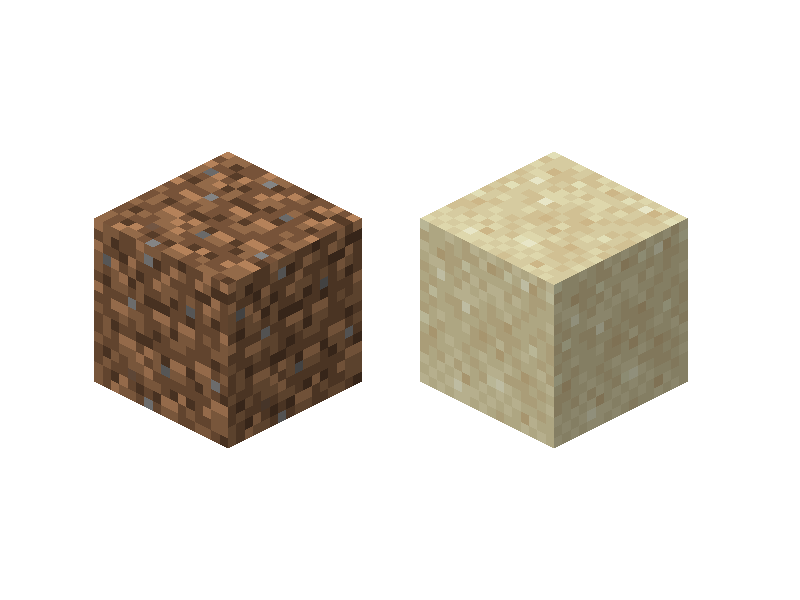
\includegraphics[scale=0.25]{staticBlock}
\caption{Dirt and Sand Block}
\end{figure}
\FloatBarrier
\item[\refstepcounter{acnum} \actheacnum \label{acDynBlocks}:] The dynamic block types including \textbf{Lava} and \textbf{Water}, shown in Figure 2, which provide explicit interactions with the game character.\\\FloatBarrier
\begin{figure}[hbt!]
\centering
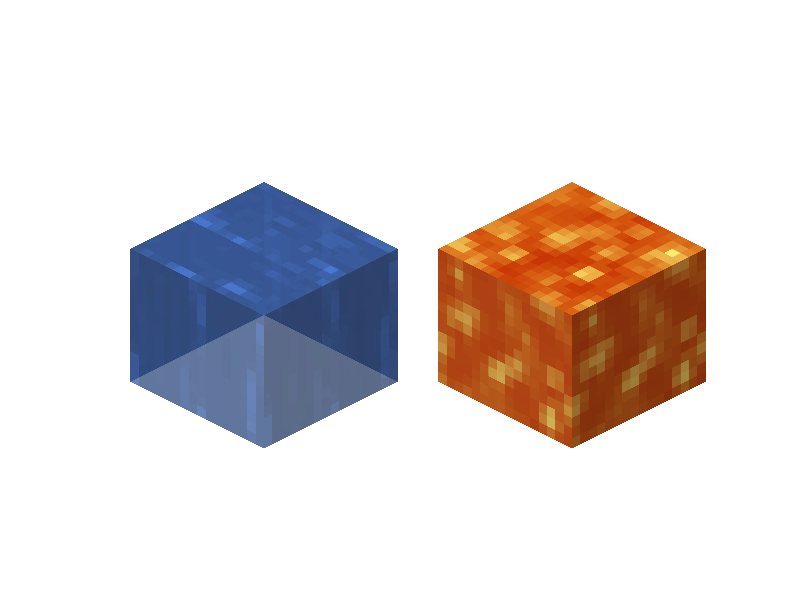
\includegraphics[scale=0.25]{block}
\caption{Lava and Water Block}
\end{figure}
\FloatBarrier

\item [\refstepcounter{acnum} \actheacnum \label{acobject}:] Objects that can interact with the game character, such as \textbf{Chicken} and \textbf{Cow}, shown in Figure 3.\\\FloatBarrier
\begin{figure}[hbt!]
\centering
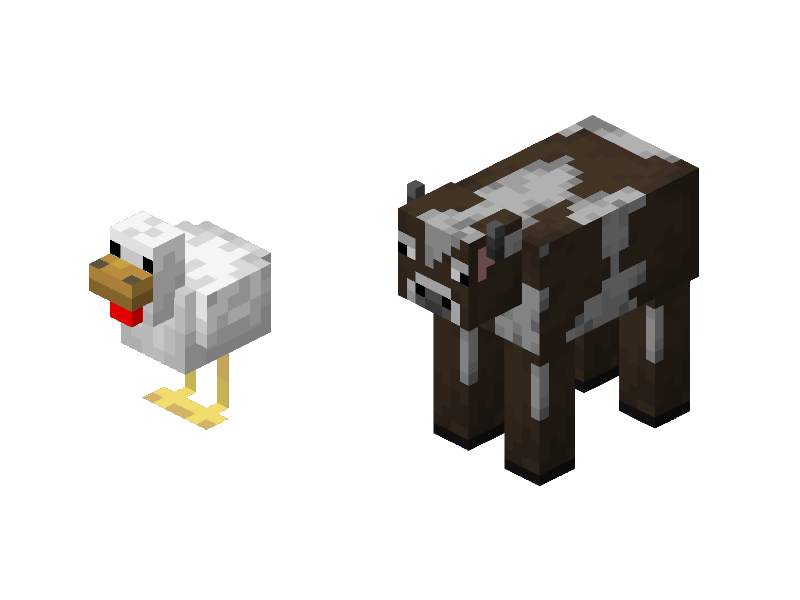
\includegraphics[scale=0.25]{object}
\caption{Chicken and Cow Object}
\end{figure}
\FloatBarrier

\item[\refstepcounter{acnum} \actheacnum \label{aiHardware}:] \textbf{Minimizing coupling: }There could be some possibilities for minimizing the coupling of the system. The current system is considered to be over decomposed and some modules are not necessary to be an individual one. Therefore, to reduce the coupling of the system, some modules can be merged into others. For example, the button module is now used by different scene modules, and those scene modules inherit the screen module. As a consequence, the button module can be merged into the screen module as part of its implementation so that the those scene modules only need to inherit the new screen module with buttons implemented within and the button module will not be needed. 
\end{description}

\subsection{Unlikely Changes} \label{SecUchange}
This section specifies the changes that are planned out but difficult to implement due to the limitation of the utilities of Pyglet.

\begin{description}
\item[\refstepcounter{ucnum} \uctheucnum \label{ucIO}:] Input Devices such as game console controller.
\item[\refstepcounter{ucnum} \uctheucnum \label{ucSave}:] Saving more game scenes, as the maximum game saving is two for now.
\item[\refstepcounter{ucnum} \uctheucnum \label{ucInventory}:] Inventory System.
\end{description}

\section{Module Hierarchy} \label{SecMH}

This section provides an overview of the module design. Modules are summarized
in a hierarchy decomposed by secrets in Table \ref{TblMH}. The Hardware-hiding section hides the hardware machine or the ``virtual machine" provided by the Pyglet. The Software decision section hides internal data structures and algorithms. The Behaviour hiding section hides input formats, screen formats, and text messages. The modules listed
below, which are leaves in the hierarchy tree, are the modules that will
actually be implemented.

\begin{description}

\item [\refstepcounter{mnum} \mthemnum \label{mHH}:] block
\item [\refstepcounter{mnum} \mthemnum \label{mHH}:] button
\item [\refstepcounter{mnum} \mthemnum \label{mHH}:] creature
\item [\refstepcounter{mnum} \mthemnum \label{mHH}:] devTools
\item [\refstepcounter{mnum} \mthemnum \label{mHH}:] game
\item [\refstepcounter{mnum} \mthemnum \label{mHH}:] loadSource
\item [\refstepcounter{mnum} \mthemnum \label{mHH}:] main
\item [\refstepcounter{mnum} \mthemnum \label{mHH}:] gameScene
\item [\refstepcounter{mnum} \mthemnum \label{mHH}:] mainScene
\item [\refstepcounter{mnum} \mthemnum \label{mHH}:] settingScene
\item [\refstepcounter{mnum} \mthemnum \label{mHH}:] player
\item [\refstepcounter{mnum} \mthemnum \label{mHH}:] processQueue
\item [\refstepcounter{mnum} \mthemnum \label{mHH}:] screen
\item [\refstepcounter{mnum} \mthemnum \label{mHH}:] shape
\item [\refstepcounter{mnum} \mthemnum \label{mHH}:] world
\end{description}

\FloatBarrier
\begin{table*}[h!]
\centering
\begin{tabular}{p{0.3\textwidth} | p{0.6\textwidth}}
\toprule
\textbf{Level 1} & \textbf{Level 2}\\
\midrule

{Hardware-Hiding Module} & \textbf{Pyglet} \\
\midrule

\multirow{7}{0.3\textwidth}{Behaviour-Hiding Module} & game\\
& gameScene\\
& mainScene\\
& settingScene\\
& player\\
& world\\
& loadSource\\
\midrule

\multirow{3}{0.3\textwidth}{Software Decision Module} & creature\\
& block\\
& screen\\
& processQueue\\
& shape\\
& devTools\\
& button\\
\bottomrule
\end{tabular}
\begin{tablenotes}
\item *Note that the main module only acts as a trigger to the program and does not support information hiding and therefore it is mentioned in either this table or Section \ref{SecMD}.
\end{tablenotes}
\caption{Module Hierarchy}
\label{TblMH}
\end{table*}
\FloatBarrier
\section{Connection Between Requirements and Design} \label{SecConnection}

The design of the system is intended to satisfy the requirements developed in
the SRS. In this stage, the system is decomposed into modules. The consistency
between requirements and modules is listed in Table \ref{TblRT}. The game module will focus on the requirements related to macro control of the GUI, menu directions, and player's input/output collection. The gameScene module will focus on the requirements related to controlling the game scene perspective captured by the player. The mainScene and settingScene modules will focus on the requirements related to menu interactions. The player module will focus on the requirements related to the character's operations and status. The world module will focus on the requirements related to loading and controlling the game world and block operations. The loadSource module will focus on the requirements related to media loading such as textures and background music. The creature module is a template module and the player module inherits it. The block module defines game blocks used by the world module. The screen module is a template module and all the scene modules inherit it. The processQueue module defines a queue to for game processes. The shape module specifies 2D and 3D coordinates locating methods. The devTools module is a development tool used by the developer to generate standard texture images. The button module will focus on the requirements related to menu buttons.


\section{Module Decomposition} \label{SecMD}

\subsection{Hardware Hiding Modules (M16)}

\begin{description}
\item[Secrets:]The algorithm used to implement the virtual hardware that controls the mouse, keyboard, monitor and audio player.
\item[Services:]Serves as a virtual hardware used by the rest of the
  system. This module provides the interface between the hardware and the
  software. So, the system can use it to display outputs or to accept inputs.
\item[Implemented By:] \textbf{OS} and \textbf{Pyglet}
\end{description}

\subsection{Behaviour-Hiding Module}
\subsubsection{game Module (M5)}
\begin{description}
\item[Secrets:]The interactive game frame(GUI).
\item[Services:]Provide the game frame(GUI) that controls the scenes switches and game world initialization.
\item[Implemented By:] game.py
\end{description}

\subsubsection{gameScene Module (M8)}
\begin{description}
\item[Secrets:]The interactive content of the game scene that will be rendered on the GUI.
\item[Services:]Render the interactive content of the game Scene on the GUI.
\item[Implemented By:] gameScene.py
\end{description}

\subsubsection{mainScene Module (M9)}
\begin{description}
\item[Secrets:]The main menu scene that will be rendered on the GUI.
\item[Services:]Render the main menu on the GUI.
\item[Implemented By:] mainScene.py
\end{description}

\subsubsection{settingScene Module (M10)}
\begin{description}
\item[Secrets:]The setting menu scene that will be rendered on the GUI.
\item[Services:]Render the setting menu on the GUI.
\item[Implemented By:] settingScene.py
\end{description}

\subsubsection{player Module (M11)}
\begin{description}
\item[Secrets:]The game character.
\item[Services:]Provide a game character with its operations in the game world.
\item[Implemented By:] player.py
\end{description}

\subsubsection{world Module (M15)}
\begin{description}
\item[Secrets:]The game world.
\item[Services:]Provide a game world and its operations.
\item[Implemented By:] world.py
\end{description}

\subsubsection{loadSource Module (M6)}
\begin{description}
\item[Secrets:]The algorithm of loading media.
\item[Services:]Provide algorithms to load texture images, background music and on-click effect sound.
\item[Implemented By:] loadSource.py
\end{description}
\subsection{Software Decision Module}

\subsubsection{screen Module (M13)}
\begin{description}
\item[Secrets:]The interactive scene template.
\item[Services:]Provide a basic template for other scenes.
\item[Implemented By:] screen.py
\end{description}

\subsubsection{creature Module (M3)}
\begin{description}
\item[Secrets:]The moving object in the game world.
\item[Services:]Provide a basic template for the moving objects in the game world.
\item[Implemented By:] creature.py
\end{description}


\subsubsection{block Module (M1)}
\begin{description}
\item[Secrets:]The game blocks.
\item[Services:]Provide a basic template for the game blocks in the game world.
\item[Implemented By:] block.py
\end{description}


\subsubsection{processQueue Module (M12)}
\begin{description}
\item[Secrets:]The processQueue data structure.
\item[Services:]Provide a data structure to store processes.
\item[Implemented By:] processQueue.py
\end{description}

\subsubsection{shape Module (M14)}
\begin{description}
\item[Secrets:]The shape drawing algorithm.
\item[Services:]Provide an algorithm to draw 2-dimensional and 3-dimensional shapes.
\item[Implemented By:] shape.py
\end{description}


\subsubsection{devTools Module (M4)}
\begin{description}
\item[Secrets:]The image process and formating algorithm.
\item[Services:]Provide an algorithm to process and produce texture images in a certain format.
\item[Implemented By:] devTools.py
\end{description}

\subsubsection{button Module (M1)}
\begin{description}
\item[Secrets:]Buttons.
\item[Services:]Provide two types of buttons(switches by OnOffButton and Toggles by Button).
\item[Implemented By:] button.py
\end{description}


\section{Traceability Matrix} \label{SecTM}

This section shows two traceability matrices: between the modules and the
requirements and between the modules and the anticipated changes.

% the table should use mref, the requirements should be named, use something
% like fref
\newpage
\begin{longtable}[h]{p{0.2\textwidth} p{0.6\textwidth}}
\toprule
\textbf{Req.} & \textbf{Modules}\\
\midrule
FR1 & M1, M2, M3, M5, M6, M7, M8, M9, M10, M11, M12, M13, M14, M15, M16\\
FR2 & M16, M5, M7, M9, M2, M14, M13\\
FR2.1 & M5, M9, M2, M16, M14\\
FR2.1.1 & M5, M9, M2, M14, M16\\
FR2.1.2 & M10, M2, M14, M15, M16\\
FR2.2 & M16, M9, M5, M2, M14\\
FR3 & M5, M11, M3\\
FR4 & M16, M8, M13, M5\\
FR4.1 & M16, M8, M13, M5\\
FR5 & M5, M8, M11, M3\\
FR5.1 & M5, M8, M11, M3\\
FR5.2 & M5, M8, M11, M3\\
FR5.3 & M5, M8, M11, M3\\
FR5.4 & M5, M8, M11, M3\\
FR6 & M5, M8, M11, M3\\
FR7 & M5, M8, M11, M3\\
FR8 & M5, M8, M11, M3\\
FR8.1 & M5, M8, M11, M3\\
FR8.2 & M5, M8, M11, M3\\
FR8.3 & M5, M8, M11, M3\\
FR9 & M16, M5, M8, M15, M11, M13, M14\\
FR10 & M5, M8, M15, M11, M12\\
FR11 & M5, M8, M15, M12, M11, M6\\
FR11.1 & M5, M8, M6\\
FR11.2 & M5, M8, M6\\
FR11.3 & M5, M8, M6\\
FR12 & M5, M16\\
FR12.1 & M5, M16, M10\\
FR12.2 & M5, M15, M14, M2, M10\\
FR12.3 & M5, M10, M2, M14\\
FR13 & M5, M10, M2, M14\\
FR14 & M7, M6, M16, M5\\
FR15 & M5, M6, M8, M16, M15, M11, M12\\
FR16 & M5, M8, M15, M11\\
FR17 & M5, M8, M6, M1\\
FR18 & M5, M8, M10, M9\\
NFR1 & M1, M2, M3, M5, M6, M7, M8, M9, M10, M11, M12, M13, M14, M15\\
NFR2 & M1, M2, M3, M5, M6, M7, M8, M9, M10, M11, M12, M13, M14, M15\\
NFR3 & M1, M2, M3, M5, M6, M7, M8, M9, M10, M11, M12, M13, M14, M15\\
NFR4 & M1, M2, M3, M5, M6, M7, M8, M9, M10, M11, M12, M13, M14, M15, M16\\
NFR5 & M1, M2, M3, M5, M6, M7, M8, M9, M10, M11, M12, M13, M14, M15, M16\\
NFR6 & M1, M2, M3, M5, M6, M7, M8, M9, M10, M11, M12, M13, M14, M15, M16\\
NFR7 & M16\\
NFR8 & M1, M2, M3, M5, M6, M7, M8, M9, M10, M11, M12, M13, M14, M15\\
NFR9 & M16\\
NFR10 & M1, M2, M3, M5, M6, M7, M8, M9, M10, M11, M12, M13, M14, M15, M16\\
NFR11 & M1, M2, M3, M5, M6, M7, M8, M9, M10, M11, M12, M13, M14, M15\\
NFR12 & M1, M2, M3, M5, M6, M7, M8, M9, M10, M11, M12, M13, M14, M15\\
NFR13 & M1, M2, M3, M5, M6, M7, M8, M9, M10, M11, M12, M13, M14, M15\\
NFR14 & M1, M2, M3, M5, M6, M7, M8, M9, M10, M11, M12, M13, M14, M15\\
\bottomrule
\caption{Trace Between Requirements and Modules}
\label{TblRT}
\end{longtable}

\begin{table}[H]
\centering
\begin{tabular}{p{0.2\textwidth} p{0.6\textwidth}}
\toprule
\textbf{AC} & \textbf{Modules}\\
\midrule
AC1 & M16\\
AC2 & M4, M6, M8, M15\\
AC3 & M4, M6, M8, M15\\
AC4 & M3, M4, M6, M8, M15\\
\bottomrule
\end{tabular}
\caption{Trace Between Anticipated Changes and Modules}
\label{TblACT}
\end{table}

\section{Use Hierarchy Between Modules} \label{SecUse}

In this section, the uses hierarchy between modules is
provided. Arrow represent USES relationship between modules.The \textbf{Hardware Hiding Module} refers to \textbf{OS} and \textbf{Pyglet} modules, which belong to external program. The figure contains two software components, \textbf{Software Game} and \textbf{Texture Image Processor}. The \textbf{Software Game} component demonstrates the use hierarchy between modules in the implementation of the game program itself. The \textbf{Texture Image Processor} is a software tool implemented by the team to produce texture images in a certain format that will be implicitly used by the block module, which is shown with a dashed arrow line.

\begin{figure}[H]
\centering
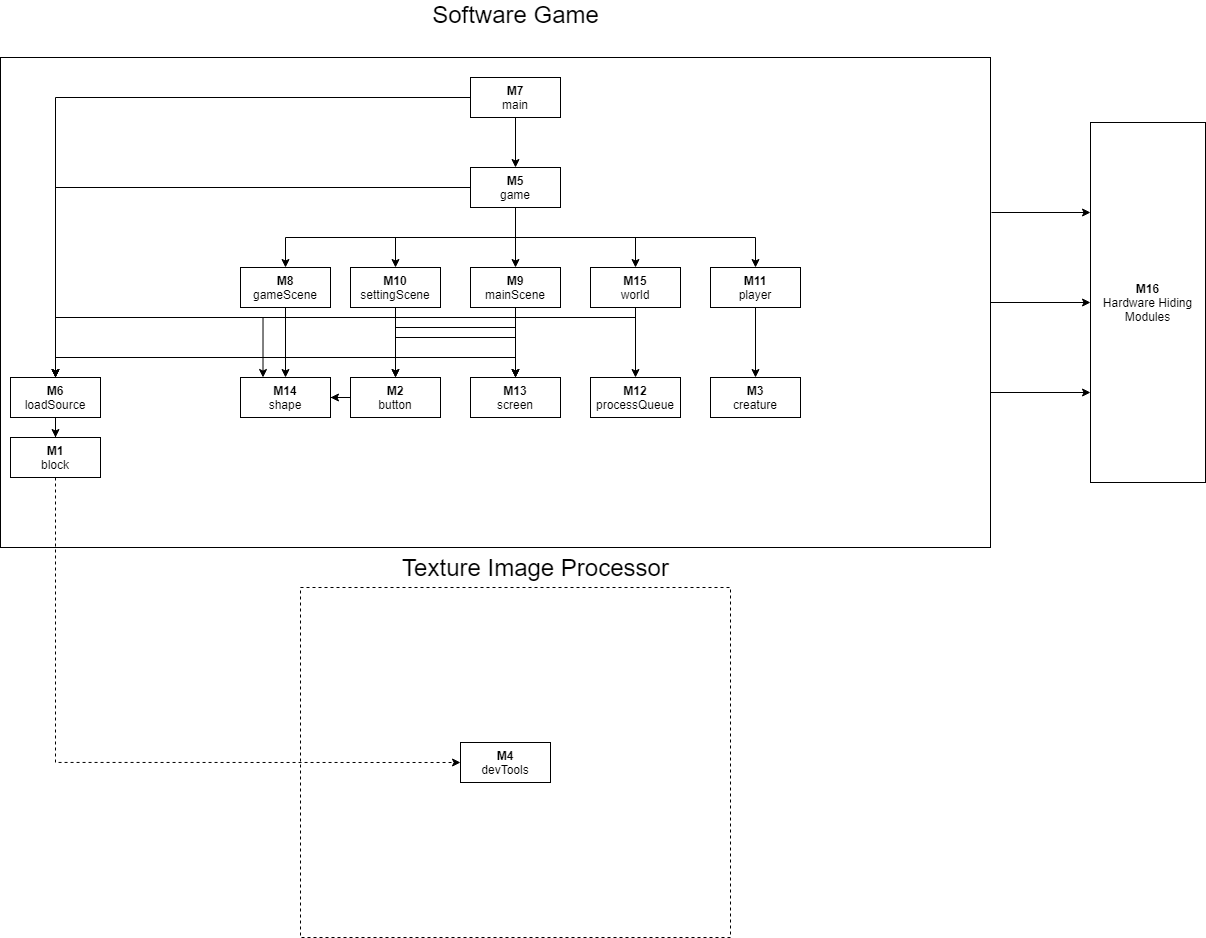
\includegraphics[width=1.05\textwidth]{use.png}
\caption{Use hierarchy among modules}
\label{FigUH}
\end{figure}

%\section*{References}

\bibliographystyle {plainnat}
\bibliography {MG}

\end{document}